\documentclass[10pt,a4paper]{article}
\usepackage[utf8]{inputenc}
\usepackage[italian]{babel}
\usepackage{amsmath}
\usepackage{amsfonts}
\usepackage{amssymb}
\usepackage{graphicx}
\usepackage[left=2cm,right=2cm,top=2cm,bottom=2cm]{geometry}
\newcommand{\rem}[1]{[\emph{#1}]}

\author{Gruppo BN \\ Federico Belliardo, Marco Costa, Lisa Bedini}
\title{Ottica 2}
\begin{document}

\maketitle
\section{Scopo dell'esperienza}
L'esperienza si divide in due parti distinte. Nella prima si stima la lunghezza d'onda della radiazione di un laser a diodo mediante la misura degli ordini di diffrazione provocati dall'incidenza sulla scala graduata di un calibro utilizzata come reticolo. Nella seconda parte mediante un laser He-Ne si calibra un interferometro di Michelson per eseguire la misura della lunghezza d'onda della riga verde del mercurio, e in seguito osservare le frange di interferenza con luce bianca.

\section{Materiale occorrente}
\begin{itemize}
\item Calibro
\item Laser a diodo
\item Metro a nastro
\item Interferometro di Michelson
\item Laser He-Ne
\item Lampada al mercurio
\item Filtro verde
\end{itemize}

\section{Parte A - Misura della lunghezza d'onda del laser a diodo}
\subsection{Modalità operative}
\begin{figure}[!htb]
  \centering
  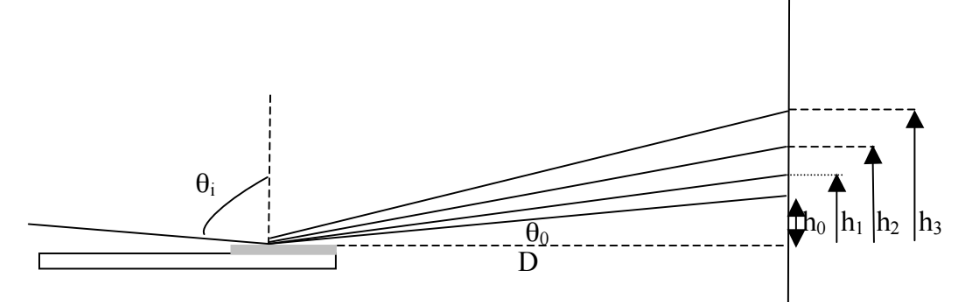
\includegraphics[scale=.5]{disegno1.png}
\caption{Disegno schematico dell'esperimento di diffrazione.}
\label{parteAfigura}

\end{figure}
La spaziatura tra le suddivisioni della scala graduata del calibro è troppo grande per poter essere usata come reticolo di diffrazione per la luce visibile senza l'accorgimento di far incidere il fascio in modo radente alla scala, cioè con angolo di incidenza prossimo a $\frac{\pi}{2}$. Il fascio riflesso e i vari ordini di diffrazione sono visibili un un muro (schermo) a circa due metro di distanza.\\
Sul muro si è posto un foglio di carta su cui si sono segnati il punto in cui il laser sarebbe arrivato se non fosse stato diffratto, il punto in cui il fascio viene riflesso dal calibro e i vari ordini di diffrazione dal calibro. La media delle posizioni del punto di incidenza diretta e del punto di riflessione è il piano del tavolo proiettato sul muro. Da questo punto è necessario misurare la distanza $D$ (distanza tra il calibro e il muro) e tutte le lunghezze $h_0, h_1, h_2,...$. indicate nella figura \ref{parteAfigura}.\\
Inserire altri eventuali accorgimenti sperimentali su come si misurano d e D e dire come sono stati presi gli errori su queste misure.\\
La misura della distanza $D$ è stata eseguito con metro a nastro, mentre per $d$ si è preso il valore nominale della separazione delle tacche della scala graduata prendendo come incertezza $frac{1}{20} mm$, cioè la suddivisone del nonio. Non sono sicuro di questa cosa.\\
\subsection{Raccolta ed elaborazione dati}
La legge del reticolo per questa configurazione geometrica è: $d(\sin  \theta_i - \sin \theta_d)  = m \lambda $, dove $\theta_d = \frac{\pi}{2} - \sin \theta_n $. Riscrivendo la legge come: $\sin \theta_d = -m \frac{\lambda}{d} + \sin \theta_i$. La relazione funzionale tra $\sin  \theta_d$ e $m$ è una retta, si è pertanto eseguito un fit dei dati riportati in tabella \ref{tabella}. Per eseguire il fit si è usata la funzione \emph{curvefit} della libreria \emph{pylab} con l'opzione \emph{$absolute\,sigma = "true"$}. Il fit della funzione lineare $y = ax+b$ ha riportato i seguenti valori: \\

Dal parametro a si riava il valore di $\lambda$ da confrontare con quello teorico del laser.

\section{Parte B - Misura della lunghezza d'onda della riga verde del mercurio}
\subsection{Calibrazione interferometro}

\begin{figure}[!htb]
  \centering
  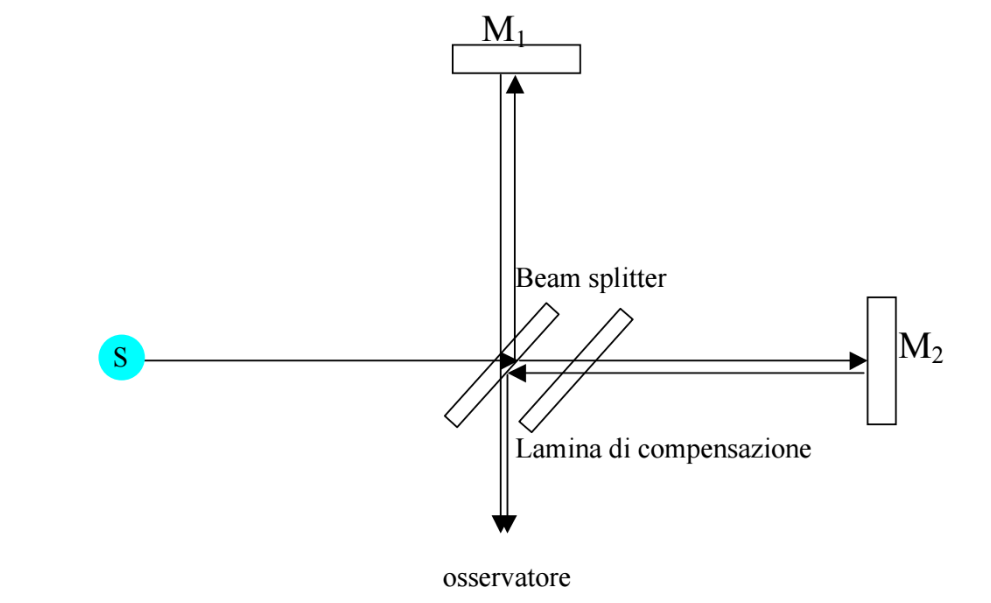
\includegraphics[scale=.5]{interferometro.png}
\caption{Disegno schematico dell'interferometro di Michelson.}
\label{parteAfigura}
\end{figure}

L'interferometro di Michelson in dotazione è dotato di una vita micrometrica che permette di spostare lo specchio $M1$ (vedi figura \ref{inferferometro}), è necessario prima misurare quale sia il rapporto tra il passo della vite e lo spostamento effettivo dello specchio, cioè misurare il fattore di demoltiplica della leva. \\
Per fare ciò si utilizza una sorgente laser He-Ne di lunghezza d'onda nota e si misura lo spostamento della vite necessario perché 30 frange passino per un certo punto dello schermo. Si sono eseguite tre misure riportate nella tabella \ref{calibrazione}, una per ognuno dei componenti del gruppo.\\

Dalla formula $2 \Delta X = m \lambda$ si è ricavato $\Delta X$ e quindi il fattore di demoltiplica $\eta = \frac{\Delta X}{\Delta s}$, dove $\Delta s$ è lo spostamento letto sulla vite micrometrica.

\subsection{Misura di lunghezza d'onda}
Si è cambiata la sorgente luminosa, si è inserita la lampada al mercurio al posto del laser He-Ne, si è aspettato il tempo sufficiente perché ci fosse termalizzazione e si è inserito il filtro verde per selezionare la riga (essere più specifici).\\
Si sono poi eseguite tre misure (una per ogni componente del gruppo) del numero di giri della vita micrometrica necessari perché 50 frange di interferenza passassero per un determinato punto dello schermo. Da queste sempre grazie alla formula precedente si è trovata la lunghezza d'onda cercata.

\section{Conclusioni}

\end{document}